\chapter{MARCO APLICATIVO}

Al ser un proyecto Open Source utilizar nombres en inglés en el desarrollo de software es preferible debido a su estandarización global en la industria. Esta práctica promueve la claridad, consistencia y accesibilidad del código, facilitando la colaboración internacional, la comprensión del código para desarrolladores futuros, y la búsqueda de recursos y documentación en línea. Además, favorece la reutilización del código en diferentes contextos y proyectos, mejorando la eficiencia y la calidad del desarrollo de software en general.

\section{Metodología de trabajo}
Las diferentes tareas se irán registrando en el tablero, a su vez, con el apoyo visual que brinda, facilita el saber en qué punto se encuentra cada actividad. Al ser un proyecto pensado para ser distribuido como Open Source, el tablero también sirve para crear nuevas Issues que cualquier contribuyente puede realizar.

A continuación, se muestra el tablero de actividades.
\begin{figure}[!h]
  \centering
  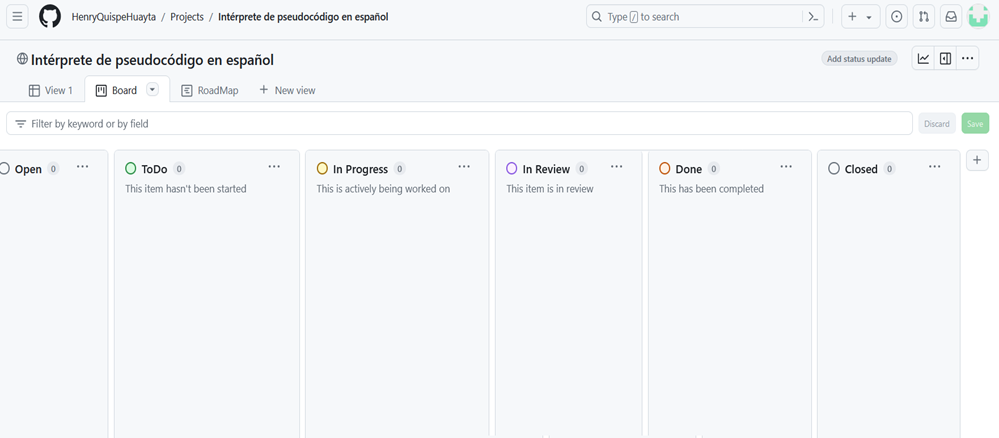
\includegraphics[width=1\textwidth]{images/tablero.png}
  \caption{Tablero de trabajo}
  \centering Fuente: Elaboración propia (GitHub)
  \label{fig:tablero}
\end{figure}
\newline
\newline
\newline

Se tiene un total de seis columnas, las cuales son:
\begin{itemize}
  \item \textbf{Open} \\
  Estas son las tareas que se han identificado inicialmente, que pueden incluir la creación de nuevas funcionalidades, corrección de errores, refactorizaciones, etc. Estas tareas están por definirse si van a ser atendidas o no. En esta etapa, se evalúa su importancia y se priorizan en función de las necesidades del proyecto.
  \item \textbf{ToDo} \\
  En esta columna del tablero se mueven las tareas que están listas para ser iniciadas. Aunque estas tareas aún no se están trabajando activamente, se encuentran en espera para su ejecución. Se aborda en función de su prioridad.
  \item \textbf{In Progress} \\
  Las tareas que se encuentran en esta columna ya están siendo trabajadas activamente. Aquí es donde se lleva a cabo la implementación de las funcionalidades o las correcciones de errores planificadas. Se monitorea el progreso de estas tareas para garantizar que avancen de manera eficiente.
  \item \textbf{In Review} \\
  Esta columna alberga las tareas que están en proceso de revisión. Una vez que una tarea ha sido completada, se somete a un proceso de revisión para garantizar la calidad del trabajo realizado. Si se encuentra algún error durante la revisión, la tarea se devuelve a la columna "In Progress" para su corrección.
  \item \textbf{Done} \\
  Una vez que una tarea ha pasado exitosamente por el proceso de revisión, se mueve a esta columna. Esto indica que la tarea ha sido completada satisfactoriamente. Las tareas permanecen en esta columna durante un tiempo antes de pasar a la columna final, en posible espera de algún cambio que requiera volver a una columna anterior.
  \item \textbf{Closed} \\
  En esta etapa final, las tareas que no requieren más trabajo o modificaciones se cierran. Esto puede incluir tareas que han sido completadas exitosamente y revisadas, así como aquellas que fueron abiertas pero finalmente decididas que no serán abordadas. Las tareas cerradas se archivan y ya no son parte del flujo de trabajo activo.
\end{itemize}

\subsection{Actividades}
Las principales actividades que se realizaron se registraron en el tablero Kanban, en la primera columna (Open).

\begin{itemize}
  \item \textbf{Implementation of Lexer (Implementación del Analizador Léxico).} \\
  Se implementó el analizador léxico del intérprete, que convirtió el código fuente en una secuencia de tokens según las reglas léxicas del lenguaje. Este componente escaneó el código y generó una lista estructurada de tokens, que fueron utilizados como entrada para las etapas posteriores del proceso de interpretación.
  \item \textbf{Implementation of Parser (Implementación del Analizador Sintáctico).} \\
  Durante esta fase, se desarrolló el analizador sintáctico que verificó la estructura gramatical del código fuente generado por el analizador léxico. El analizador sintáctico transformó la secuencia de tokens en un árbol de sintaxis abstracta (AST), asegurando que el código siguiera las reglas sintácticas del intérprete.
  \item \textbf{Interpreter Development and Code Execution (Desarrollo del Intérprete y Ejecución de Código).} \\
  Se completó la implementación del intérprete que utilizó el AST generado por el analizador sintáctico para ejecutar el programa. El intérprete interpretó cada nodo del AST y ejecutó las operaciones definidas por el código fuente, facilitando la ejecución del programa en tiempo real. \\
  \item \textbf{Error Handling (Manejo de Errores).} \\
  Durante esta etapa, se implementó un sistema completo de manejo de errores que detectó y gestionó problemas como errores de sintaxis, referencias a variables no definidas, y operaciones inválidas. Se proporcionaron mensajes de error detallados y personalizados para mejorar la experiencia del usuario y facilitar la depuración del código.
  \item \textbf{Context and Scope Management (Gestión de Contexto y Ámbito).} \\
  Se definió y se implementó cómo se almacenaron y accedieron variables y funciones dentro de diferentes contextos durante la ejecución del programa. La gestión adecuada de ámbitos aseguró que las variables locales y globales se manejan correctamente, contribuyendo a la correcta ejecución y funcionamiento del intérprete.
  \item \textbf{Definition of Built-in Constants and Values (Definición de Constantes y Valores Integrados).} \\
  Como fase final, se definieron y se implementaron las palabras clave, funciones integradas, constantes predefinidas y mensajes de error estándar del lenguaje. Estos elementos proporcionan la base fundamental para la funcionalidad básica del intérprete, permitiendo a los usuarios utilizar y gestionar de manera efectiva los recursos del lenguaje de programación implementado.
\end{itemize}

\begin{figure}[!h]
  \centering
  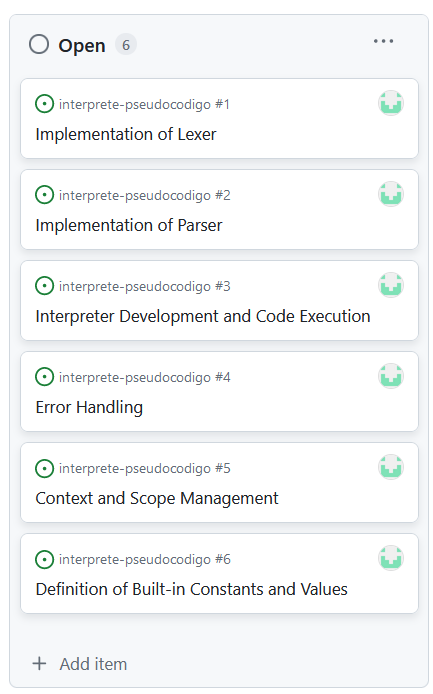
\includegraphics[width=0.6\textwidth]{images/actividades.png}
  \caption{Actividades realizadas}
  \centering Fuente: Elaboración propia (GitHub)
  \label{fig:actividades}
\end{figure}

\section{Análisis léxico}
\subsection{Lexemas y tokens}
Los Lexemas son el conjunto de palabras reservadas, signos, operadores y separadores, las palabras reservadas son palabras clave que no se pueden utilizar como identificadores, los signos y operadores sirven para realizar las operaciones y los separadores nos permiten indicar dónde comienza y termina cada uno de nuestros lexemas y la gramática en sí.
\begin{center}
  \begin{longtable}{|l|m{10em}|m{14em}|}
    \hline
    \textbf{Token} & \textbf{Descripción} & \textbf{Estructura o Formato Esperado} \\
    \hline
    \endfirsthead
    \hline
    \endhead
    \endfoot
    \hline
    TT\_INT & Tipo de dato entero & Números entero en base 10 \\
    \hline
    TT\_FLOAT & Tipo de dato real & Número decimal con punto flotante \\
    \hline
    TT\_STRING & Tipo de dato cadena & Cadena delimitada por comillas dobles \\
    \hline
    TT\_IDENTIFIER & Identificador & Nombres de variables y funciones \\
    \hline
    TT\_KEYWORD & Palabra clave & Palabra reservada del lenguaje \\
    \hline
    TT\_PLUS & Operador suma & Signo + \\
    \hline
    TT\_MINUS & Operador suma & Signo - \\
    \hline
    TT\_MUL & Operador multiplicación & Signo * \\
    \hline
    TT\_DIV & Operador división & Signo / \\
    \hline
    TT\_MOD & Operador módulo & Signo \% \\
    \hline
    TT\_POW & Operador potencia & Operador de potencia, ** \\
    \hline
    TT\_EQ & Operador igualdad & Operador de asignación o igualdad, = \\
    \hline
    TT\_LPAREN & Paréntesis izquierdo & Paréntesis de apertura, ( \\
    \hline
    TT\_RPAREN & Paréntesis derecho & Paréntesis de cierre, ) \\
    \hline
    TT\_LSQUARE & Corchete izquierdo & Corchete de apertura, [ \\
    \hline
    TT\_RSQUARE & Corchete derecho & Corchete de cierre, ] \\
    \hline
    TT\_EE & Operador igualdad estricta & Operador de comparación estricta de igualdad, == \\
    \hline
    TT\_MM & Operador decremento & Operador de decremento, -- \\
    \hline
    TT\_NE &Operador no igual &Operador de comparación de no igualdad, != \\
    \hline
    TT\_LT & Operador menor que & Operador de comparación menor que, < \\
    \hline
    TT\_GT & Operador mayor que & Operador de comparación mayor que, > \\
    \hline
    TT\_LTE & Operador menor o igual que & Operador de comparación menor o igual que, <= \\
    \hline
    TT\_GTE & Operador mayor o igual que & Operador de comparación mayor o igual que, >= \\
    \hline
    TT\_COMMA & Coma & Carácter de coma , \\
    \hline
    TT\_NEWLINE & Nueva línea & Carácter de salto de línea, \textbackslash n \\
    \hline
    TT\_EOF & Fin de archivo & N/A \\
    \hline
    \caption{Tokens. Tipos básicos}
  \end{longtable}
  \vspace*{-2.5em}
  \centering Fuente: Elaboración propia
\end{center}

Además de los tokens básicos, están las palabras reservadas específicas del intérprete:
\begin{table}[!h]
  \begin{center}
    \begin{tabularx}{0.9\textwidth}{|X|X|X|}
      \hline
      \textbf{Lexema} & \textbf{Descripción} & \textbf{Palabra Clave} \\
      \hline
      var & Variable & var \\
      \hline
      print & Mostrar en consola & imprimir \\
      \hline
      if & Condición si & si \\
      \hline
      then & Instrucción entonces & entonces \\
      \hline
      else & Instrucción sino & sino \\
      \hline
      elif & Instrucción osi & osi \\
      \hline
      end & Fin condición si & fin \\
      \hline
      while & Bucle mientras & mientras \\
      \hline
      then & Instrucción entonces & entonces \\
      \hline
      end & Fin bucle mientras & fin \\
      \hline
      in & Instrucción hasta & hasta \\
      \hline
      for & Bucle para & para \\
      \hline
      end & Fin bucle para & fin \\
      \hline
      function & Inicio función & funcion \\
      \hline
      end & Fin función & fin \\
      \hline
    \end{tabularx}
  \end{center}
  \caption{Lexemas y palabras reservadas}
  \centering Fuente: Elaboración propia
  \label{tab:lexemas}
\end{table}

\subsection{Autómatas individuales}
Los autómatas individuales son utilizados para representar gráficamente la secuencia de caracteres de las palabras reservadas, los signos y los operadores de nuestra gramática. Cada tipo de token puede ser representado mediante un autómata finito que define su estructura.

A continuación, en la Tabla \ref{tab:automatas}, se presentan los autómatas individuales para los tipos de tokens básicos del intérprete. Cada autómata describe la estructura y el formato esperado de los lexemas correspondientes, lo que permite identificar y clasificar los tokens durante el análisis léxico.
\begin{center}
  \begin{longtable}{|l|l|}
    \hline
    \multicolumn{1}{|l|}{\textbf{Tipo de Token}} & \multicolumn{1}{l|}{\textbf{Descripción Token}} \\
    \hline
    \endfirsthead
    \hline
    \endhead
    \hline
    \endfoot
    \endlastfoot
    TT\_INT, TT\_FLOAT & Tipo de dato entero y real \\
    \hline
    \multicolumn{2}{|l|}{} \\
    \multicolumn{2}{|c|}{
      \begin{minipage}{0.95\textwidth}
        \centering
        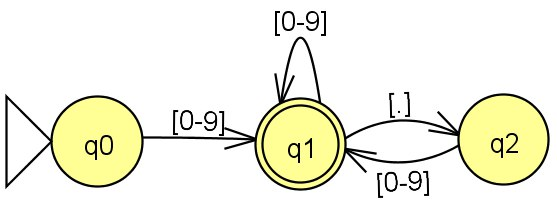
\includegraphics[width=0.6\textwidth]{images/number.png} \\[2ex]
        \begin{math}
          \begin{array}{rl}
            q0 & = [0-9] \, q1 \\
            q1 & = [0-9]^{*} + [.] \, q2 + \lambda \\
            q2 & = [0-9] \\
            ER & = [0-9]([0-9]+[.][0-9])^{*}
          \end{array}
        \end{math}
      \end{minipage}
    } \\
    \multicolumn{2}{|l|}{Estado inicial: q0} \\
    \multicolumn{2}{|l|}{
      \begin{minipage}{0.9\textwidth
      }
        \textbf{Transiciones:}
        \vspace*{-0.8em}
        \begin{itemize}
          \item Desde el estado q0 se requiere un dígito $([0-9])$ para poder pasar al estado q1.
          \item En el estado q1, puede haber un número indefinido de dígitos $([0-9])$ y finalizar sin pasar al estado q2.
          \item Puede haber un punto decimal $(.)$ que lleva al estado q2.
          \item En el estado q2, debe haber al menos un dígito $([0-9])$ después del punto decimal $(.)$ que lleva al estado q1.
        \end{itemize}
      \end{minipage}
    } \\
    \multicolumn{2}{|l|}{Estado final: q1 es el estado final válido.} \\
    \hline
    TT\_STRING & Tipo de dato cadena \\
    \hline
    \multicolumn{2}{|l|}{} \\
    \multicolumn{2}{|c|}{
      \begin{minipage}{0.95\textwidth}
        \centering
        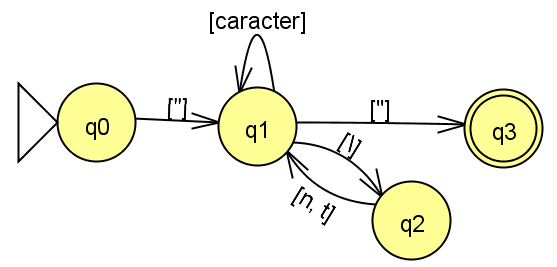
\includegraphics[width=0.6\textwidth]{images/string.png} \\[2ex]
        \begin{math}
          \begin{array}{rl}
            q0 & = ["] \, q1 \\
            q1 & = [caracter] q1 + [\backslash] \, q2 + ["] \, q3 \\
            q2 & = ([n] + [t]) \, q1 \\
            q3 & = \lambda \\
            ER & = ["]([caracter])^{*} ["] \, + \\
            & \quad ["][caracter]^{*} [\backslash] (([t]+[n])[caracter]^{*}[\backslash])^{*} ([t]+[n])[caracter]^{*} ["]
          \end{array}
        \end{math}
      \end{minipage}
    } \\
    \multicolumn{2}{|l|}{Estado inicial: q0} \\
    \multicolumn{2}{|l|}{
      \begin{minipage}{0.9\textwidth
      }
        \textbf{Transiciones:}
        \vspace*{-1.5em}
        \begin{itemize}
          \item Comienza con una comilla doble $(")$, pasa al estado q1.
          \item En el estado q1, puede haber cualquier carácter $([caracter])$, seguido por más caracteres o secuencias de escape como \textbackslash n o \textbackslash t.
          \item Se permite un número indefinido de repeticiones de caracteres y secuencias de escape.
          \item Termina con otra comilla doble $(")$, llegando al estado final q3.
        \end{itemize}
      \end{minipage}
    } \\
    \multicolumn{2}{|l|}{Estado final: q3 es el estado final válido.} \\
    \hline
    TT\_EQ, TT\_EE & Operador igualdad y comparación estricta \\
    \hline
    \multicolumn{2}{|l|}{} \\
    \multicolumn{2}{|c|}{
      \begin{minipage}{0.95\textwidth}
        \centering
        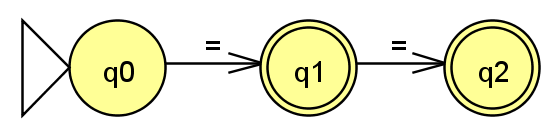
\includegraphics[width=0.6\textwidth]{images/equal.png} \\[2ex]
        \begin{math}
          \begin{array}{rl}
            q0 & = [=] \, q1 \\
            q1 & = ([=] + \lambda)\, q2 \\
            q2 & = \lambda \\
            ER & = [=]([=] + \lambda)
          \end{array}
        \end{math}
      \end{minipage}
    } \\
    \multicolumn{2}{|l|}{Estado inicial: q0} \\
    \multicolumn{2}{|l|}{
      \begin{minipage}{0.9\textwidth
      }
        \textbf{Transiciones:}
        \vspace*{-1.5em}
        \begin{itemize}
          \item Un solo símbolo de igual (=) lleva al estado final q1.
        \end{itemize}
      \end{minipage}
    } \\
    \multicolumn{2}{|l|}{Estado final: q2 es el estado final válido.} \\
    \hline
    TT\_NE & Operador no igual \\
    \hline
    \multicolumn{2}{|l|}{} \\
    \multicolumn{2}{|c|}{
      \begin{minipage}{0.95\textwidth}
        \centering
        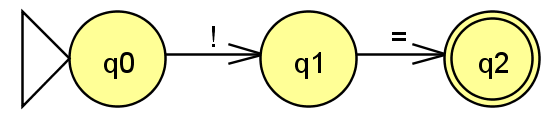
\includegraphics[width=0.6\textwidth]{images/notEqual.png} \\[2ex]
        \begin{math}
          \begin{array}{rl}
            q0 & = [!] \, q1 \\
            q1 & = [=] \, q2 \\
            q2 & = \lambda \\
            ER & = [!][=]
          \end{array}
        \end{math}
      \end{minipage}
    } \\
    \multicolumn{2}{|l|}{Estado inicial: q0} \\
    \multicolumn{2}{|l|}{
      \begin{minipage}{0.9\textwidth
      }
        \textbf{Transiciones:}
        \vspace*{-1.5em}
        \begin{itemize}
          \item Un signo de exclamación (!) seguido de un signo de igual (=) lleva al estado final q2.
        \end{itemize}
      \end{minipage}
    } \\
    \multicolumn{2}{|l|}{Estado final: q2 es el estado final válido.} \\
    \hline
    TT\_GT, TT\_GTE & Operador mayor que y mayor o igual que \\
    \hline
    \multicolumn{2}{|l|}{} \\
    \multicolumn{2}{|c|}{
      \begin{minipage}{0.95\textwidth}
        \centering
        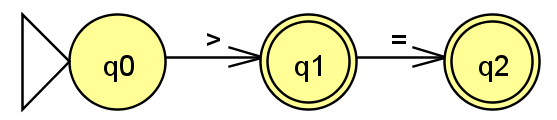
\includegraphics[width=0.6\textwidth]{images/greater.png} \\[2ex]
        \begin{math}
          \begin{array}{rl}
            q0 & = [>] \, q1 \\
            q1 & = ([=] + \lambda) \, q2 \\
            q2 & = \lambda \\
            ER & = [>]([=] + \lambda)
          \end{array}
        \end{math}
      \end{minipage}
    } \\
    \multicolumn{2}{|l|}{Estado inicial: q0} \\
    \multicolumn{2}{|l|}{
      \begin{minipage}{0.9\textwidth
      }
        \textbf{Transiciones:}
        \vspace*{-1.5em}
        \begin{itemize}
          \item Un solo signo de mayor que (>), seguido opcionalmente de un signo de igual (=), lleva al estado final q2.
        \end{itemize}
      \end{minipage}
    } \\
    \multicolumn{2}{|l|}{Estado final: q2 es el estado final válido.} \\
    \hline
    TT\_LT, TT\_LTE & Operador menor que y menor o igual que \\
    \hline
    \multicolumn{2}{|c|}{
      \begin{minipage}{0.95\textwidth}
        \centering
        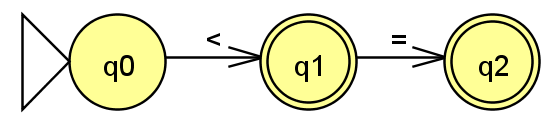
\includegraphics[width=0.6\textwidth]{images/less.png} \\[2ex]
        \begin{math}
          \begin{array}{rl}
            q0 & = [<] \, q1 \\
            q1 & = ([=] + \lambda) \, q2 \\
            q2 & = \lambda \\
            ER & = [<]([=] + \lambda)
          \end{array}
        \end{math}
      \end{minipage}
    } \\
    \multicolumn{2}{|l|}{Estado inicial: q0} \\
    \multicolumn{2}{|l|}{
      \begin{minipage}{0.9\textwidth
      }
        \textbf{Transiciones:}
        \vspace*{-1.5em}
        \begin{itemize}
          \item Un solo signo de menor que (<), seguido opcionalmente de un signo de igual (=), lleva al estado final q2.
        \end{itemize}
      \end{minipage}
    } \\
    \multicolumn{2}{|l|}{Estado final: q2 es el estado final válido.} \\
    \hline
    \caption{Autómatas individuales}
    \label{tab:automatas}
  \end{longtable}
  \vspace*{-2.5em}
  \centering Fuente: Elaboración propia
\end{center}

\section{Análisis sintáctico}
\subsection{Gramática BNF}
Cada regla de la gramática BNF se compone de símbolos no terminales y terminales, donde los símbolos no terminales representan categorías sintácticas que pueden expandirse en otras reglas, mientras que los símbolos terminales son los elementos léxicos fundamentales del lenguaje.

Para las distintas Palabras claves (Keywords) que tiene el intérprete sus gramáticas serían las siguientes:

\begin{itemize}
  \item \textbf{IF-THEN-END} \\
  \begin{math}
    \begin{array}{rl}
      <instruccion> & ::= Keywords.IF <expresion> Keywords.THEN \\ 
        & \quad <lista\_instrucciones> Keywords.END
    \end{array}
  \end{math} \\
  Define una estructura condicional que comienza con si, seguida de una condición $(<expresion>)$, un bloque de instrucciones $(<lista\_instrucciones>)$ y termina con fin. Se usa para ejecutar un bloque de código si se cumple una condición.
  \item \textbf{ELSEIF y ELSE} \\
  \begin{math}
    \begin{array}{rl}
      <caso> & ::= Keywords.ELSEIF <expresion> Keywords.THEN \\
        & \quad <lista\_instrucciones> <inst\_parar> \\
      <caso> & ::= Keywords.ELSE : <lista\_instrucciones> <inst\_parar>
    \end{array}
  \end{math} \\
  ELSEIF se utiliza para añadir una condición alternativa a una estructura IF, mientras que ELSE se usa para ejecutar un bloque de código si ninguna de las condiciones anteriores se cumple.
  \item \textbf{FOR-TO-STEP} \\
  \begin{math}
    \begin{array}{rl}
      <inst\_para> & ::= Keywords.FOR <inst\_asignacion> Keywords.TO \\
        & \quad <expresion> [Keywords.STEP <expresion>] \\ 
        & \quad Keywords.THEN <lista\_instrucciones> \\
        & \quad Keywords.END
    \end{array}
  \end{math} \\
  Define un bucle for que inicializa una variable $(<inst\_asignacion>)$, especifica una condición de terminación $(TO <expresion>)$, y opcionalmente un paso $(STEP <expresion>)$, ejecutando un bloque de código repetidamente hasta que se cumpla la condición de terminación.
  \item \textbf{WHILE-END} \\
  \begin{math}
    \begin{array}{rl}
      <inst\_mientras> & ::= Keywords.WHILE <expresion> \\
        & \quad Keywords.THEN <lista\_instrucciones> \\
        & \quad Keywords.END
    \end{array}
  \end{math} \\
  Define un bucle while que ejecuta un bloque de código mientras se cumpla una condición $(<expresion>)$, terminando cuando la condición ya no se cumple.
  \item \textbf{FUNCTION-END} \\
  \begin{math}
    \begin{array}{rl}
      <inst\_funcion> & ::= Keywords.FUNCTION <identificador> \\
        & \quad Keywords.THEN <lista\_instrucciones> \\
        & \quad Keywords.END
    \end{array}
  \end{math} \\
  Define la estructura que comienza con función, seguida de un $(<identificador>)$, un bloque de instrucciones $(<lista\_instrucciones>)$ y termina con fin. Se utiliza para definir una función personalizada que puede ser llamada en otras partes del código.
  \item \textbf{VAR} \\
  \begin{math}
    \begin{array}{rl}
      <inst\_variable> & ::= Keywords.VAR <identificador> \\
      & \quad Keywords.EQ <expresion>
    \end{array}
  \end{math} \\
  Define una instrucción de asignación que comienza con var, seguida de un $(<identificador>)$, un signo de igualdad $(Keywords.EQ)$ y una $(<expresion>)$ que se asigna a la variable.
  \item \textbf{RETURN} \\
  \begin{math}
    \begin{array}{rl}
      <inst\_retorno> & ::= Keywords.RETURN <expresion>
    \end{array}
  \end{math} \\
  Define una instrucción de retorno que comienza con return, seguida de una $(<expresion>)$ que se devuelve como resultado de la función o para salir de un bucle.
  \item \textbf{CONTINUE y BREAK} \\
  \begin{math}
    \begin{array}{rl}
      <inst\_continuar> & ::= Keywords.CONTINUE \\
      <inst\_parar> & ::= Keywords.BREAK
    \end{array}
  \end{math} \\
  CONTINUE se utiliza para saltar a la siguiente iteración de un bucle, mientras que BREAK se usa para salir de un bucle antes de que se complete.
  \item \textbf{PRINT} \\
  \begin{math}
    \begin{array}{rl}
      <inst\_imprimir> & ::= Keywords.PRINT (<expresion>)
    \end{array}
  \end{math} \\
  Define una instrucción de impresión que comienza con imprimir, seguida de una $(<expresion>)$ que se muestra en la consola.
\end{itemize}

\subsection{Primeros}
Los primeros de una gramática son los símbolos no terminales que pueden aparecer en la parte izquierda de una producción. Los primeros determinan qué símbolos pueden comenzar una cadena derivada de un símbolo no terminal. Para la gramática del intérprete, los primeros de cada no terminal son los siguientes:
\begin{table}[!h]
  \begin{center}
    \begin{tabularx}{1\textwidth}{|X|X|}
      \hline
      \textbf{No Terminal} & \textbf{Primeros} \\
      \hline
      <instruccion> & Keywords.IF, Keywords.WHILE, Keywords.FOR, Keywords.FUNCTION, Keywords.VAR, Keywords.RETURN, Keywords.CONTINUE, Keywords.BREAK, Keywords.PRINT, Identificador \\
      \hline
      <caso> & Keywords.ELSEIF, Keywords.ELSE \\
      \hline
      <inst\_para> & Keywords.FOR \\
      \hline
      <inst\_mientras> & Keywords.WHILE \\
      \hline
      <inst\_funcion> & Keywords.FUNCTION \\
      \hline
      <inst\_variable> & Keywords.VAR \\
      \hline
      <inst\_retorno> & Keywords.RETURN \\
      \hline
      <inst\_continuar> & Keywords.CONTINUE \\
      \hline
      <inst\_parar> & Keywords.BREAK \\
      \hline
      <inst\_imprimir> & Keywords.PRINT \\
      \hline
    \end{tabularx}
  \end{center}
  \caption{Primeros de la gramática}
  \centering Fuente: Elaboración propia
  \label{tab:primeros}
\end{table}

\subsection{Siguientes}
Los siguientes de una gramática son los símbolos no terminales que pueden aparecer inmediatamente después de un símbolo no terminal en una cadena derivada. Los siguientes determinan qué símbolos pueden seguir a un no terminal en una derivación. Para la gramática del intérprete, los siguientes de cada no terminal son los siguientes:
\begin{table}[!h]
  \begin{center}
    \begin{tabularx}{1\textwidth}{|X|X|}
      \hline
      \textbf{No Terminal} & \textbf{Siguientes} \\
      \hline
      <instruccion> & Keywords.END, Identificador \\
      \hline
      <caso> & Keywords.END, Keywords.ELSEIF, Keywords.ELSE \\
      \hline
      <inst\_para> & Keywords.END, Identificador \\
      \hline
      <inst\_mientras> & Keywords.END, Identificador \\
      \hline
      <inst\_funcion> & Keywords.END, Identificador \\
      \hline
      <inst\_variable> & Keywords.END, Identificador \\
      \hline
      <inst\_retorno> & Keywords.END, Identificador \\
      \hline
      <inst\_continuar> & Keywords.END, Identificador \\
      \hline
      <inst\_parar> & Keywords.END, Identificador \\
      \hline
      <inst\_imprimir> & Keywords.END, Identificador \\
      \hline
    \end{tabularx}
  \end{center}
  \caption{Siguientes de la gramática}
  \centering Fuente: Elaboración propia
  \label{tab:siguientes}
\end{table}

\section{Análisis semántico}
El análisis semántico es una etapa crucial en el proceso de compilación e interpretación que verifica la corrección semántica del código fuente después de haber pasado por el análisis léxico y sintáctico. La implementación del análisis semántico se realizó siguiendo estos puntos:

\subsection{Definición de Contextos y Alcance}
\begin{itemize}
  \item Se definieron contextos que guardan información sobre el alcance actual, incluyendo variables, funciones y otros identificadores visibles.
  \item Los contextos permitieron la gestión de scopes, soportando características como variables locales y globales, y la resolución de nombres.
\end{itemize}

\subsection{Verificación de Tipos}
\begin{itemize}
  \item Se implementaron reglas para verificar que las operaciones realizadas sobre los datos fueran semánticamente válidas. Por ejemplo, no se permitía sumar una cadena con un número.
  \item Se verificó que las funciones se llamaran con los tipos y cantidad correctos de argumentos.
\end{itemize}

\section{Evaluación y Ejecución}
\subsection{Evaluación}
El intérprete lee y analiza el contenido del archivo .inf. Durante este proceso, identifica y carga todas las variables, funciones y configuraciones definidas en el archivo. Este paso asegura que todos los elementos necesarios para la ejecución del programa estén disponibles.

Verifica las reglas semánticas definidas internamente y aplicadas en el archivo .inf. Por ejemplo, puede asegurarse de que las variables estén correctamente declaradas y que las funciones estén bien definidas según las reglas gramaticales y semánticas del intérprete.

\subsection{Ejecución}
Una vez completada la evaluación semántica y cargadas todas las configuraciones necesarias desde el archivo .inf, el intérprete procede a ejecutar el programa principal.

El intérprete ejecuta las instrucciones secuenciales definidas en el programa principal. Durante este proceso, el intérprete puede modificar el estado de las variables, realizar cálculos, llamar a funciones definidas previamente, y mostrar información en pantalla.

Una vez que todas las instrucciones del programa principal han sido ejecutadas, el intérprete completa su ejecución. En este punto, puede devolver un resultado final al usuario, mostrar información en pantalla, o realizar cualquier acción definida por el programa.

Durante la ejecución, el intérprete también maneja posibles errores que puedan surgir, como errores de sintaxis, errores de tiempo de ejecución (como divisiones por cero o acceso a memoria no válida), o excepciones específicas del lenguaje. La gestión adecuada de errores asegura que el programa pueda responder de manera apropiada ante situaciones inesperadas.
